\let\negmedspace\undefined
\let\negthickspace\undefined
\documentclass[journal,12pt,twocolumn]{IEEEtran}
\usepackage{cite}
\usepackage{amsmath,amssymb,amsfonts,amsthm}
\usepackage{algorithmic}
\usepackage{graphicx}
\usepackage{textcomp}
\usepackage{xcolor}
\usepackage{txfonts}
\usepackage{listings}
\usepackage{enumitem}
\usepackage{mathtools}
\usepackage{gensymb}
\usepackage[breaklinks=true]{hyperref}
\usepackage{tkz-euclide} % loads  TikZ and tkz-base
\usepackage{listings}
%\usepackage{gvv}
%
%\usepackage{setspace}
%\usepackage{gensymb}
%\doublespacing
%\singlespacing

%\usepackage{graphicx}
%\usepackage{amssymb}
%\usepackage{relsize}
%\usepackage[cmex10]{amsmath}
%\usepackage{amsthm}
%\interdisplaylinepenalty=2500
%\savesymbol{iint}
%\usepackage{txfonts}
%\restoresymbol{TXF}{iint}
%\usepackage{wasysym}
%\usepackage{amsthm}
%\usepackage{iithtlc}
%\usepackage{mathrsfs}
%\usepackage{txfonts}
%\usepackage{stfloats}
%\usepackage{bm}
%\usepackage{cite}
%\usepackage{cases}
%\usepackage{subfig}
%\usepackage{xtab}
%\usepackage{longtable}
%\usepackage{multirow}
%\usepackage{algorithm}
%\usepackage{algpseudocode}
%\usepackage{enumitem}
%\usepackage{mathtools}
%\usepackage{tikz}
%\usepackage{circuitikz}
%\usepackage{verbatim}
%\usepackage{tfrupee}
%\usepackage{stmaryrd}
%\usetkzobj{all}
%    \usepackage{color}                                            %%
%    \usepackage{array}                                            %%
%    \usepackage{longtable}                                        %%
%    \usepackage{calc}                                             %%
%    \usepackage{multirow}                                         %%
%    \usepackage{hhline}                                           %%
%    \usepackage{ifthen}                                           %%
  %optionally (for landscape tables embedded in another document): %%
%    \usepackage{lscape}     
%\usepackage{multicol}
%\usepackage{chngcntr}
%\usepackage{enumerate}

%\usepackage{wasysym}
%\documentclass[conference]{IEEEtran}
%\IEEEoverridecommandlockouts
% The preceding line is only needed to identify funding in the first footnote. If that is unneeded, please comment it out.

\newtheorem{theorem}{Theorem}[section]
\newtheorem{problem}{Problem}
\newtheorem{proposition}{Proposition}[section]
\newtheorem{lemma}{Lemma}[section]
\newtheorem{corollary}[theorem]{Corollary}
\newtheorem{example}{Example}[section]
\newtheorem{definition}[problem]{Definition}
\newcommand{\solution}{\noindent \textbf{Solution: }}
%\newtheorem{thm}{Theorem}[section] 
%\newtheorem{defn}[thm]{Definition}
%\newtheorem{algorithm}{Algorithm}[section]
%\newtheorem{cor}{Corollary}
\newcommand{\BEQA}{\begin{eqnarray}}
\newcommand{\EEQA}{\end{eqnarray}}
\newcommand{\define}{\stackrel{\triangle}{=}}
\theoremstyle{remark}
\newtheorem{rem}{Remark}
\let\vec\mathbf
\newcommand{\myvec}[1]{\ensuremath{\begin{pmatrix}#1\end{pmatrix}}}
%\bibliographystyle{ieeetr}
\usepackage{graphicx}
\begin{document}
%

\bibliographystyle{IEEEtran}


\vspace{3cm}

\title{
%	\logo{
ASSIGNEMNT-1 PROBABILITY
}
\author{ Katherapaka Nikhil EE22BTECH11028$^{*}$% <-this % stops a space 
}	


\maketitle

\newpage

%\tableofcontents

\bigskip

\renewcommand{\thefigure}{\theenumi}
\renewcommand{\thetable}{\theenumi}



Question 1.27\\
Verify that
$\vec{A}-\vec{F}=\vec{E}-\vec{D}$ \\
The quadrilateral AFDE is defined\\ 
to be a parallelogram.\\
\solution:
D,E,F are midpoints of BC,CA,AB respectively
\begin{align}
\vec{D}&=\frac{1}{2}\myvec{-4-3 \\ 6-5}\\
&=\frac{1}{2}\myvec{-7 \\ 1}\\
\vec{E}&=\frac{1}{2}\myvec{1-3 \\ -1-5}\\
&=\frac{1}{3}\myvec{-2 \\ 6}\\
\vec{F}&=\frac{1}{2}\myvec{1-4 \\ -1+6}\\
&=\frac{1}{3}\myvec{-3 \\ 5}\\
\vec{A}-\vec{F}&=\frac{1}{2}\myvec{2+3 \\ -2-5}\\
&=\frac{1}{2}\myvec{5 \\ -7}\\
\vec{E}-\vec{D}&=\frac{1}{2}\myvec{-2+7 \\ -6-1}\\
&=\frac{1}{2}\myvec{5 \\ -7}\\
\therefore{}&\vec{A-F=E-D}
\end{align}
%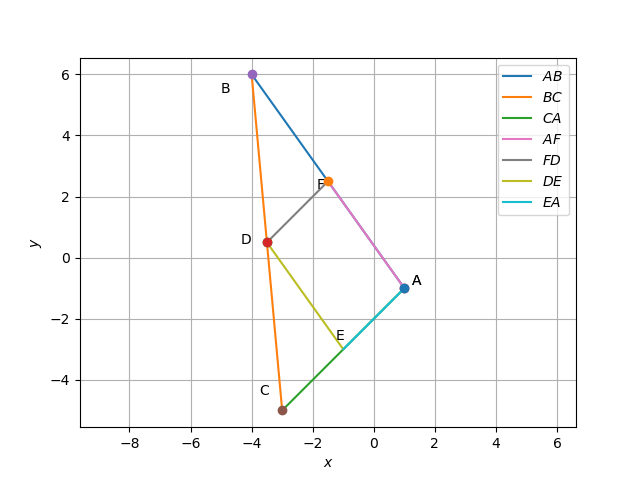
\includegraphics[scale=0.4]{image2}
\begin{figure}[t]
\centering
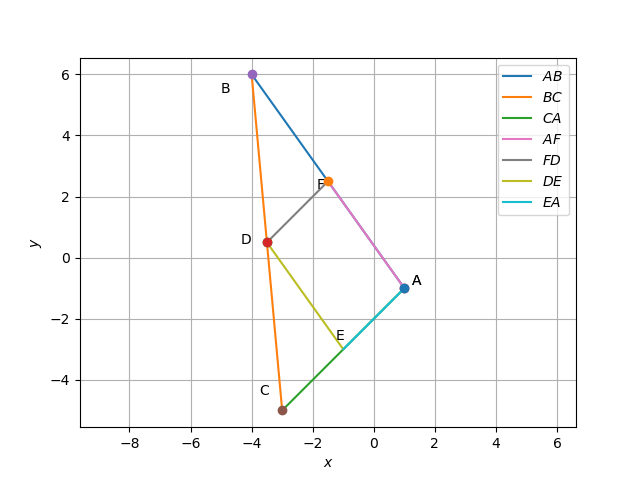
\includegraphics[width=\columnwidth]{image2}
\caption{The quadrilateral AFDE is defined to be a parallelogram.}
\label{fig:image2}
\end{figure}
%Fig. \ref{fig:image2} ABC is a Triangle
\end{document}
